The constant $c_s$ model was chosen as the model to test PTtools with,
as the model is the next logical extension of the bag model,
and there is some reference data available from \cites{giese_2020}{giese_2021}.
Figure \ref{fig:fluid_profiles} demonstrates solutions for three different wall speeds $v_\text{wall}$ and two different transition strengths $\alpha_n$ of eq. \eqref{eq:alpha_n}.
% These are not the same as the values \cite[fig. 10]{hindmarsh_gw_pt_2019}.
Instead of using only the bag model which has the squared sound speeds $c_{s,s}^2 = c_{s,b}^2 = \frac{1}{3}$,
each plot has four curves, each corresponding to a different combination of the squared sound speeds
$c_{s,s}^2 \in \{ \frac{1}{3}, \frac{1}{4} \}, c_{s,b}^2 \in \{ \frac{1}{3}, \frac{1}{4} \}$.
The corresponding gravitational wave spectra are plotted in figure \ref{fig:gw_spectra}.
Converting these to the frequencies and amplitudes today results in figure \ref{fig:omgw0},
which also contains the LISA instrument noise spectrum as a reference.

\begin{figure}[ht!]
\centering
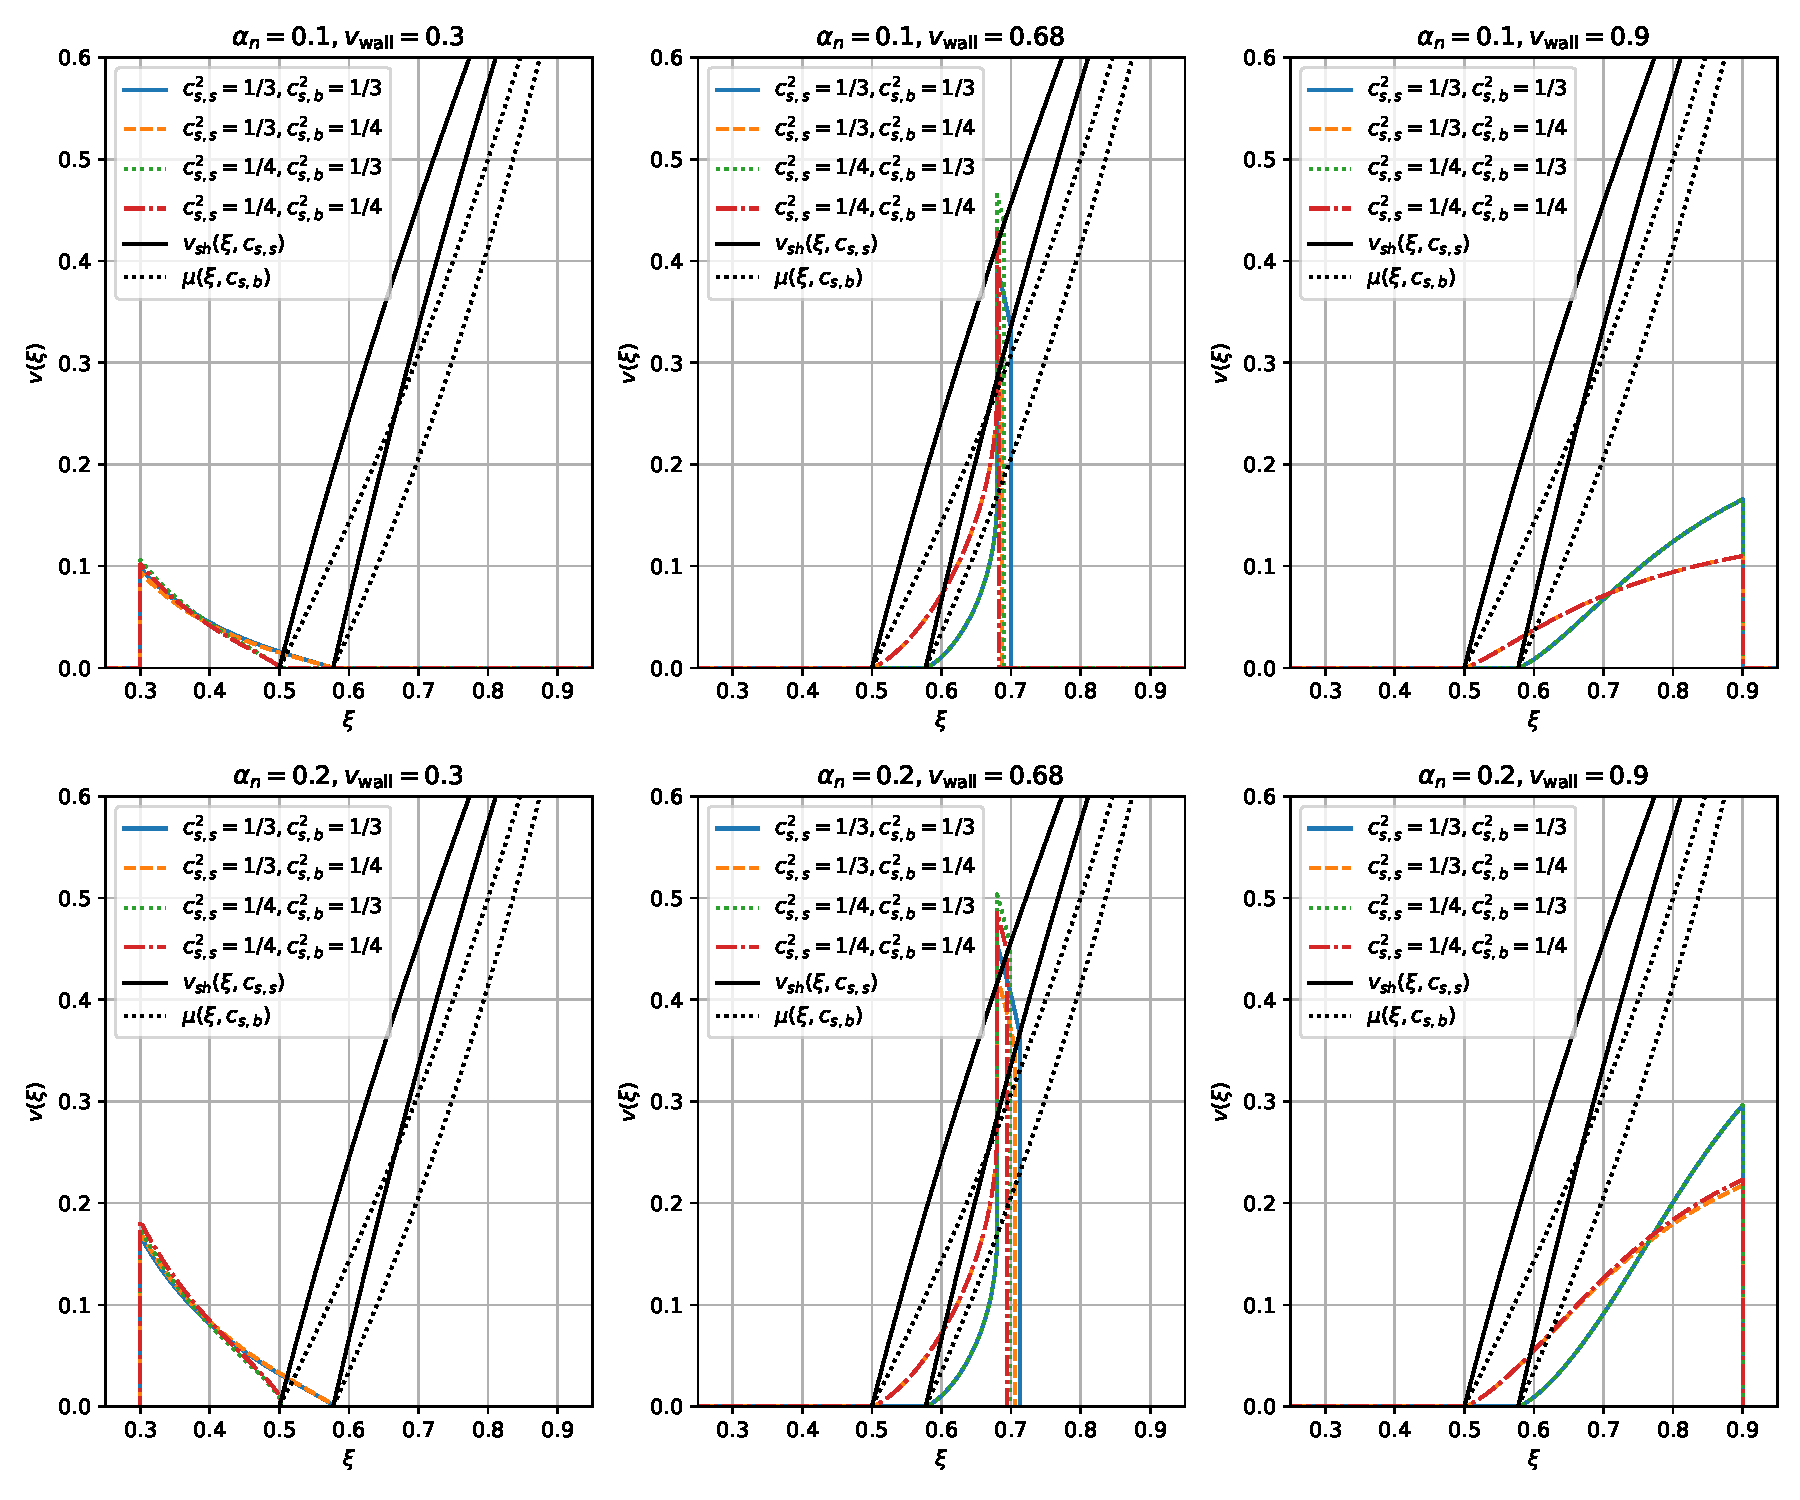
\includegraphics[width=\textwidth]{fig/const_cs_gw_v.pdf}
\caption{Self-similar fluid profiles with four sound speed combinations, three different wall speeds $v_\text{wall}$ and two transition strengths $\alpha_n$}
\label{fig:fluid_profiles}
\end{figure}

\begin{figure}[ht!]
\centering
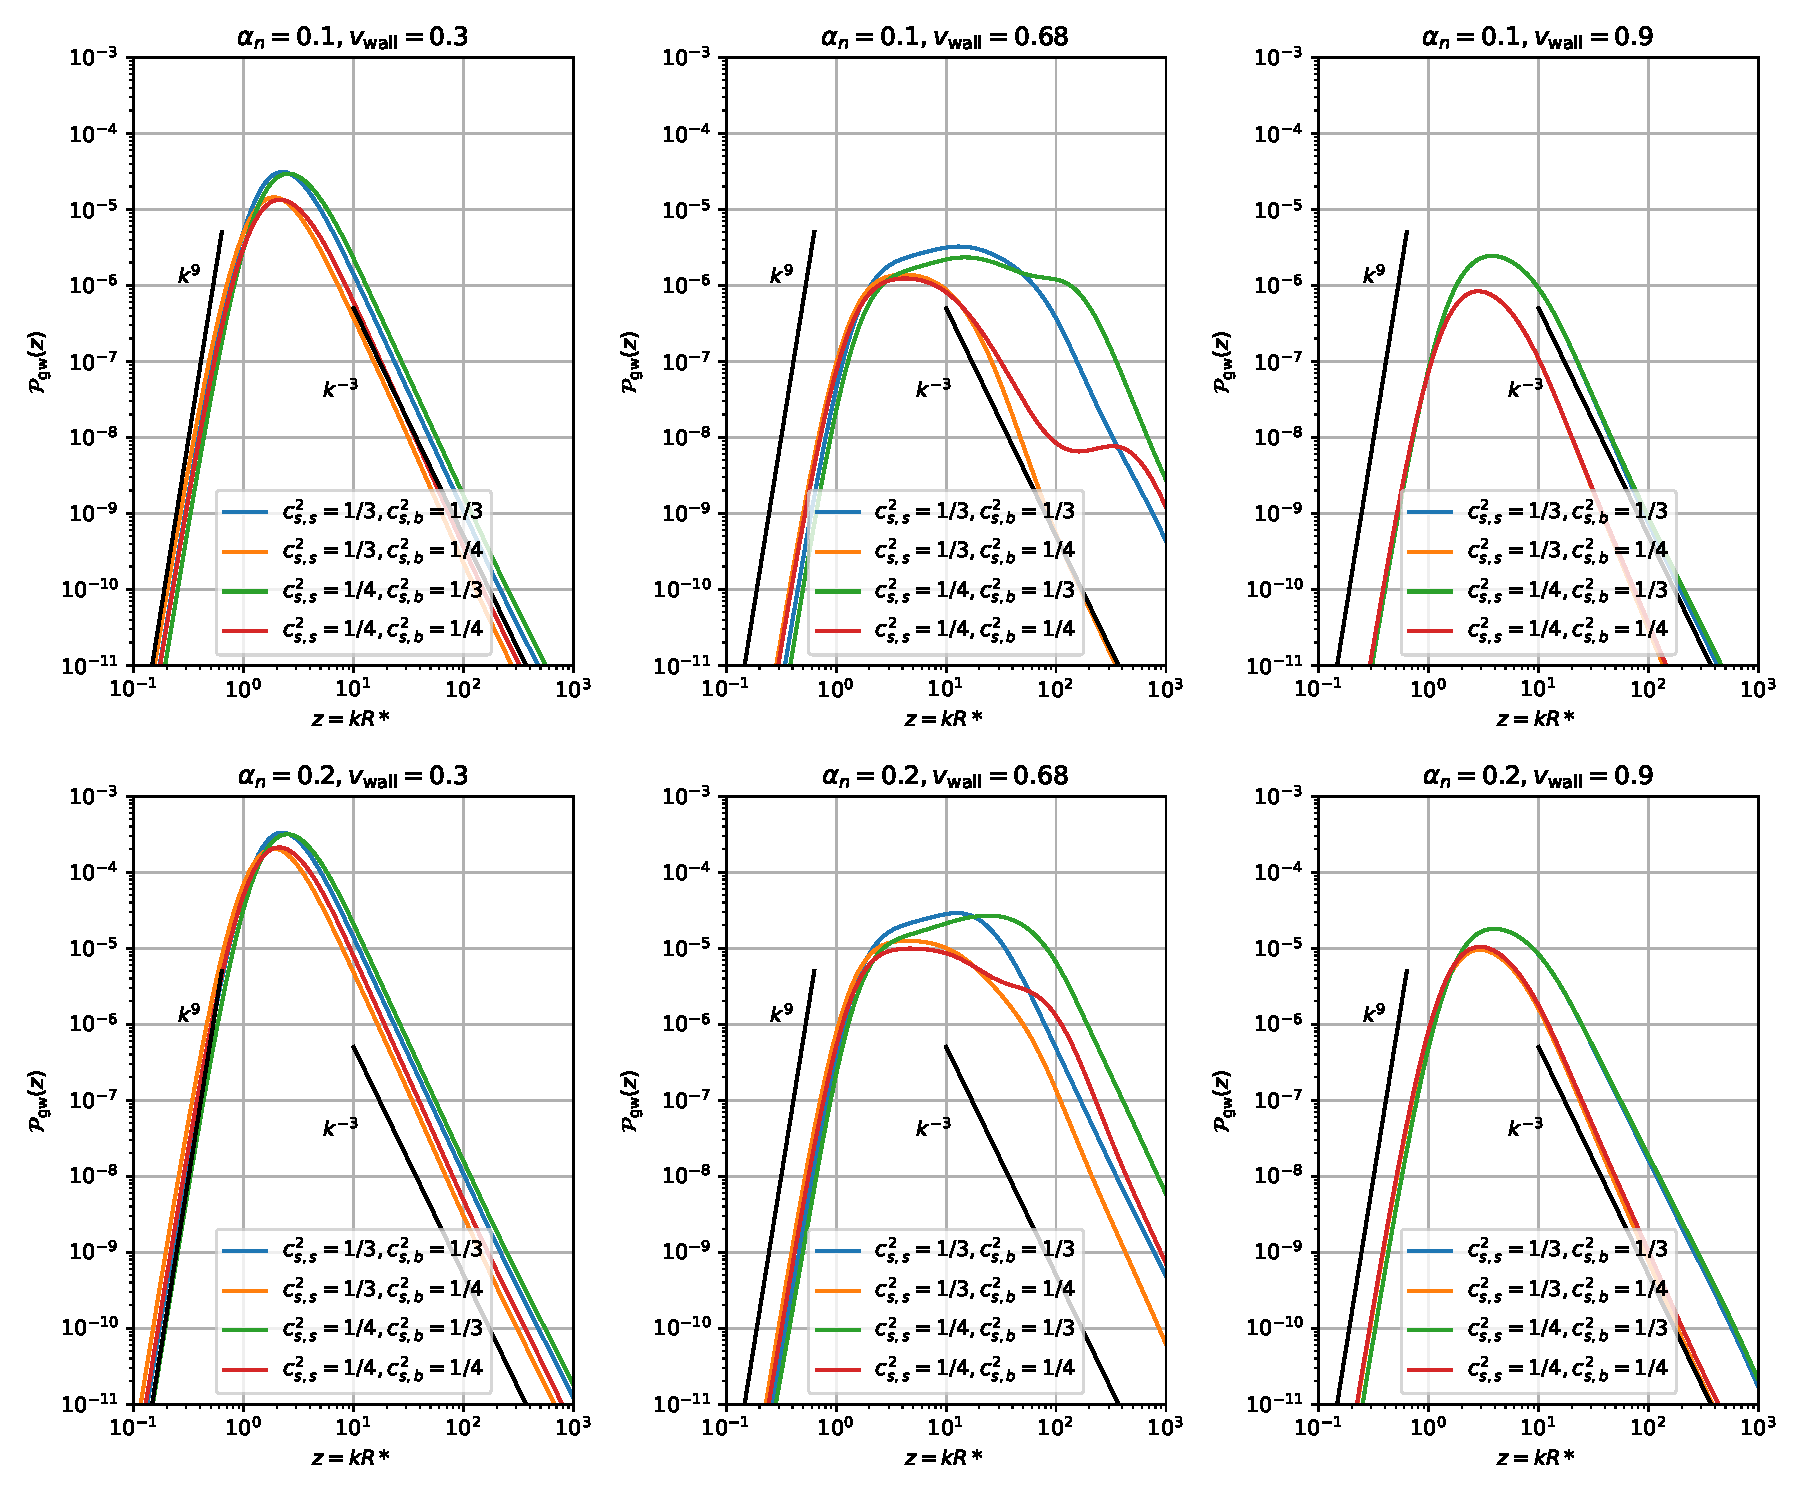
\includegraphics[width=\textwidth]{fig/const_cs_gw.pdf}
\caption{Gravitational wave power spectra computed with the sound shell model from the fluid profiles of fig. \ref{fig:fluid_profiles}}
\label{fig:gw_spectra}
\end{figure}

\begin{figure}[ht!]
\centering
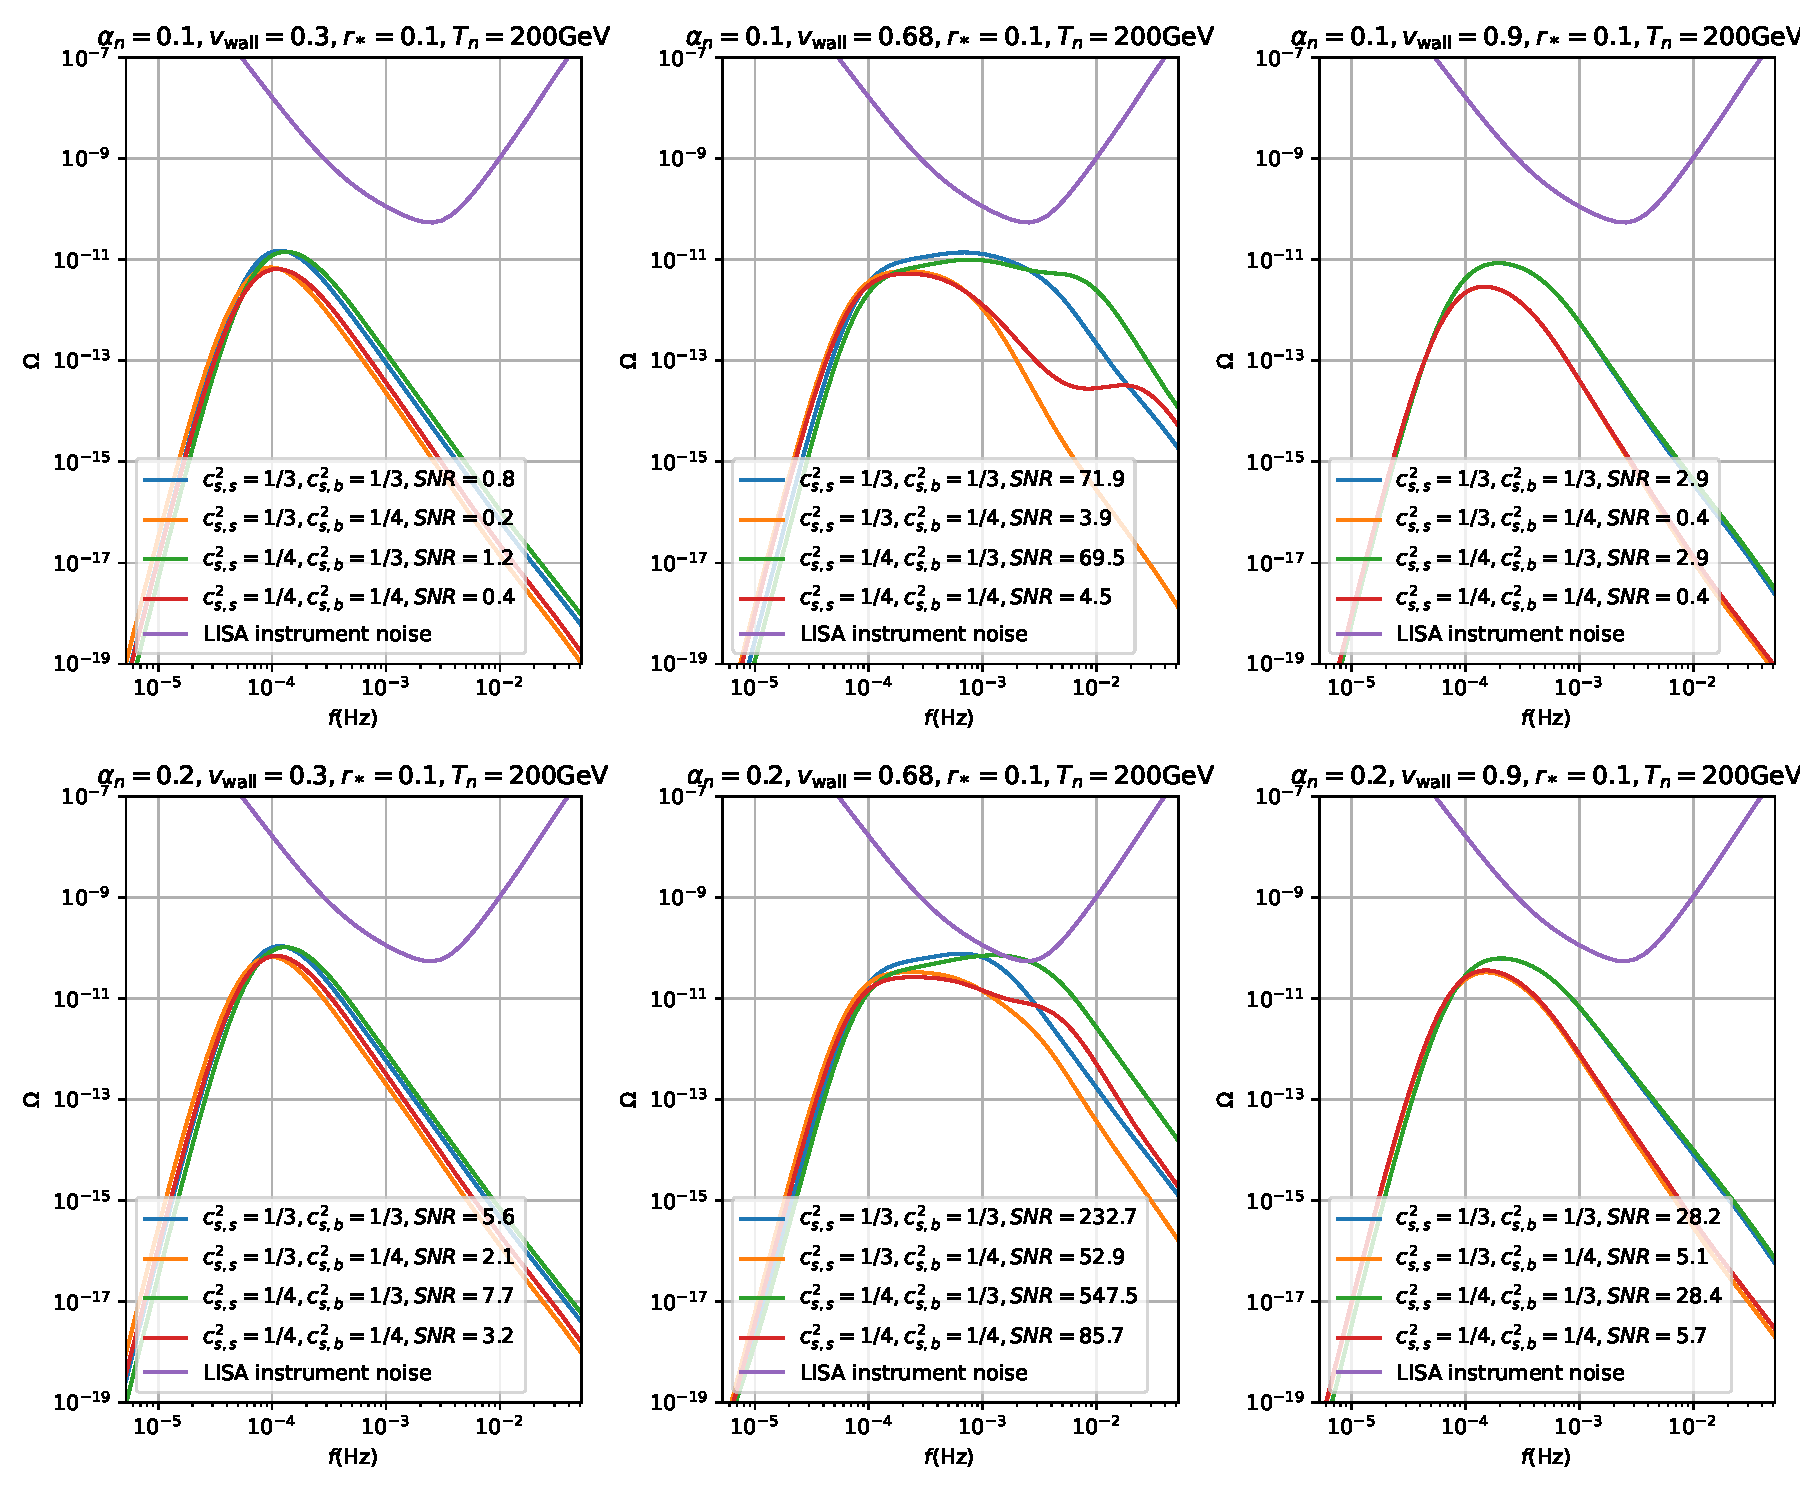
\includegraphics[width=\textwidth]{fig/const_cs_gw_omgw0.pdf}
\caption{Scaled gravitational wave power spectra today, $\Omega_{gw,0}$, of the gravitational wave power spectra of fig. \ref{fig:gw_spectra}}
\label{fig:omgw0}
\end{figure}

\iffalse
\begin{table}
\centering
\caption{Signal-to-noise ratios of the gravitational wave power spectra of fig \ref{fig:omgw0}}
\begin{tabular}{l|l|l|l}
Model & \multicolumn{3}{l}{$\v_\text{wall}$} \\
& 0.30 & 0.68 & 0.90
\hline \\
$c_{s,s}^2=1/3, c_{s,b}^2=1/3$ & 0.8 & 71.9 & 2.9 \\
$c_{s,s}^2=1/3, c_{s,b}^2=1/4$ & 0.2 & 3.9 & 0.4 \\
$c_{s,s}^2=1/4, c_{s,b}^2=1/3$ & 1.2 & 69.5 & 2.9 \\
$c_{s,s}^2=1/4, c_{s,b}^2=1/4$ & 0.4 & 4.5 & 0.4 \hline \\
$c_{s,s}^2=1/3, c_{s,b}^2=1/3$ & 5.6 & 232.7 & 28.2 \\
$c_{s,s}^2=1/3, c_{s,b}^2=1/4$ & 2.1 & 52.9 & 5.1 \\
$c_{s,s}^2=1/4, c_{s,b}^2=1/3$ & 7.7 & 547.5 & 28.4 \\
$c_{s,s}^2=1/4, c_{s,b}^2=1/4$ & 3.2 & 85.7 & 5.7 \\
\end{tabular}
\label{table:const_cs_gw_snr}
\end{table}

\fi

These figures demonstrate that the sound speed can have a profound effect on the resulting gravitational wave spectrum.
To understand how the sound speed affects the gravitational wave spectrum,
we have to first study the fluid shells of figure \ref{fig:fluid_profiles}.
There are two curves that constrain the shape of the fluid shells.
The solid black curves are the shock velocities $v_\text{sh}(\xi,c_{s,s})$ that are determined by $c_{s,s}$.
In general the shock velocity is also dependent on the enthalpy density $w$, since $c_s = c_s(w,\phi)$,
but in the constant sound speed model the sound speed is independent of the enthalpy,
as it is a constant for each phase.
Therefore we can plot the shock velocities as curves in the 2D plots instead of having to plot them as surfaces as functions of $(\xi,w)$ in a 3D plot.
The dotted black curves are the $\mu(\xi,c_{s,b})$ curves of eq. \eqref{eq:mu} that constrain the maximum fluid velocity inside the bubble.
They are dependent on the choice of $c_{s,b}$.
The $v_\text{sh}$ curves encounter $v=0$ at $\xi = c_{s,s}$ and the $\mu$ curves at $\xi = c_{s,b}$.

For all solution types, adjusting either of the sound speeds affects the degrees of freedom and therefore the pressure $p$ and enthalpy density $w$ for that phase.
This affects the solution of the bubble wall junction conditions of eq. \eqref{eq:junction_condition_1}, \eqref{eq:junction_condition_2} and therefore $v(\xi_\text{wall})$,
which is also the peak of the fluid velocity profile.
This effect can be seen at the top-left figure, where all four fluid shells have different $v(\xi_\text{wall})$.
The change caused by adjusting the sound speed is the most profound for deflagrations when $c_{s,s}$ is decreased below $v_\text{wall}$, as it causes them to become hybrids, and vice versa.
Similarly changing $c_{s,b}$ so that the Chapman-Jouguet speed of \eqref{eq:chapman_jouguet} is decreased below $v_\text{wall}$ converts a hybrid to a detonation, and vice versa.

For deflagrations and hybrids, adjusting $c_{s,s}$ affects the location of the shock and therefore the thickness of the fluid shell.
It also affects the ODE group of eq. \eqref{eq:hydro_param1}, \eqref{eq:hydro_param2}, \eqref{eq:hydro_param3} and therefore the shape of the fluid shell in front of the bubble wall.
These effects can be seen at the top-left and bottom-left figures, where the curves with the same $c_{s,s}$ are grouped together.
Correspondingly for hybrids, adjusting $c_{s,b}$ affects $\mu(\xi_\text{wall},c_{s,b})$,
which is the point from which the integration of the detonation-like part of the fluid shell starts.
This can be seen in the two figures at the middle, where the detonation-like tails of the curves with the same $c_{s,b}$ are grouped together.
And for both detonations and hybrids, adjusting $c_{s,b}$ affects the shape of the fluid shell behind the wall.

These differences in the shapes of the fluid shells carry over to the gravitational wave spectra of fig. \ref{fig:gw_spectra} and eventually of the gravitational wave spectra today in fig. \ref{fig:omgw0}.
The sine transformation of eq. \eqref{eq:ssm_f} and \eqref{eq:ssm_l} in the process converts the fluid shells of fig. \ref{fig:fluid_profiles} to the gravitational wave spectra of \ref{fig:gw_spectra} has the same basic properties as a Fourier transform.
Therefore, by comparing the fluid velocity profiles and the gravitational wave spectra we can identify a few general correlations.
The thinner the fluid shell is, the broader the gravitational wave spectrum.
And the higher the fluid velocities are in the fluid shell, the higher is the intensity of the gravitational waves.
Thin shells also have more of the higher frequencies.
These effects can be seen in the case of thin hybrids of the middle figures.
Hybrids consist of two sections with significantly differing characteristics.
Therefore, the hybrids and especially the thin hybrids with high fluid velocities in front of the wall have a gravitational wave spectrum with two distinct contributions.
This results in a significantly higher gravitational wave spectrum in the higher frequencies resulting in a significantly higher signal-to-noise ratio (SNR),
which distinguishes them from the detonations and deflagrations.
% However, regarding hybrids and especially these thin hybrids
% it should be noted that the hybrid solutions are very finely tuned, and may not exist in a real fluid.
% \cite[p. 5]{gowling_lisa_2021}
Outside the region of the peak, the gravitational wave spectra follow a $k^9$ power law at low $z$,
and $k^{-3}$ at high $z$.

The signal-to-noise ratios of the example spectra in figure \ref{fig:omgw0}
are entirely below the LISA noise curve except for the one curve with
$c_{s,s} = \frac{1}{4}, c_{s,b} = \frac{1}{3}, \alpha_n = 0.2, v_\text{wall} = 0.68$,
but the signal-to-noise ratios above unity by an order of magnitude or two for many of the curves.
This is thanks to the integrated nature of the signal,
which makes the overall signal distinguishable from the noise power spectrum even though the power at individual frequencies is below the noise.
\cite{thrane_sensitivity_2013}

% -----
% Giese comparison
% -----

To test the precision and reliability of the results provided by PTtools,
we compared to the results given by the code in  Giese et al., 2021 \cite[fig. 2]{giese_2021}.
The reference fluid profiles are generated by the in the article,
and the $\kappa$ of eq. \eqref{eq:kappa_omega} is computed by PTtools.
The resulting $\kappa$ values are in fig. \ref{fig:kappa_giese},
and the relative differences in fig. \ref{fig:kappa_giese_diff}
The colors from blue to gray correspond to $\alpha = 0.01, 0.03, 0.1, 0.3, 1, 3$.
For each color, the solid line has $c_{s,s}^2 = \frac{1}{3}, c_{s,b}^2 = \frac{1}{3}$,
the dashed line has $c_{s,s}^2 = \frac{1}{3}, c_{s,b}^2 = \frac{1}{4}$,
the dotted line has $c_{s,s}^2 = \frac{1}{4}, c_{s,b}^2 = \frac{1}{3}$
and the dot-dashed line has $c_{s,s}^2 = \frac{1}{4} c_{s,b}^2 = \frac{1}{4}$.

\begin{figure}[ht!]
\centering
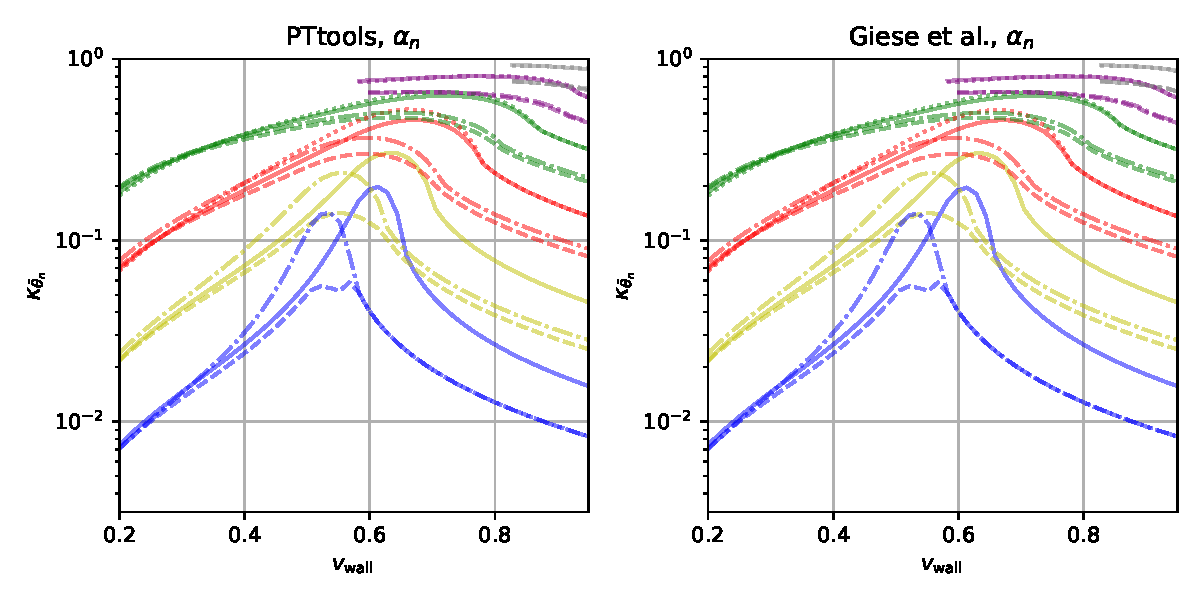
\includegraphics[width=\textwidth]{fig/giese_lisa_fig2_alpha_n.pdf}
\caption{Comparison of $\kappa$ values by \cite[fig. 2]{giese_2021} and PTtools}
\label{fig:kappa_giese}
\end{figure}

\begin{figure}[ht!]
\centering
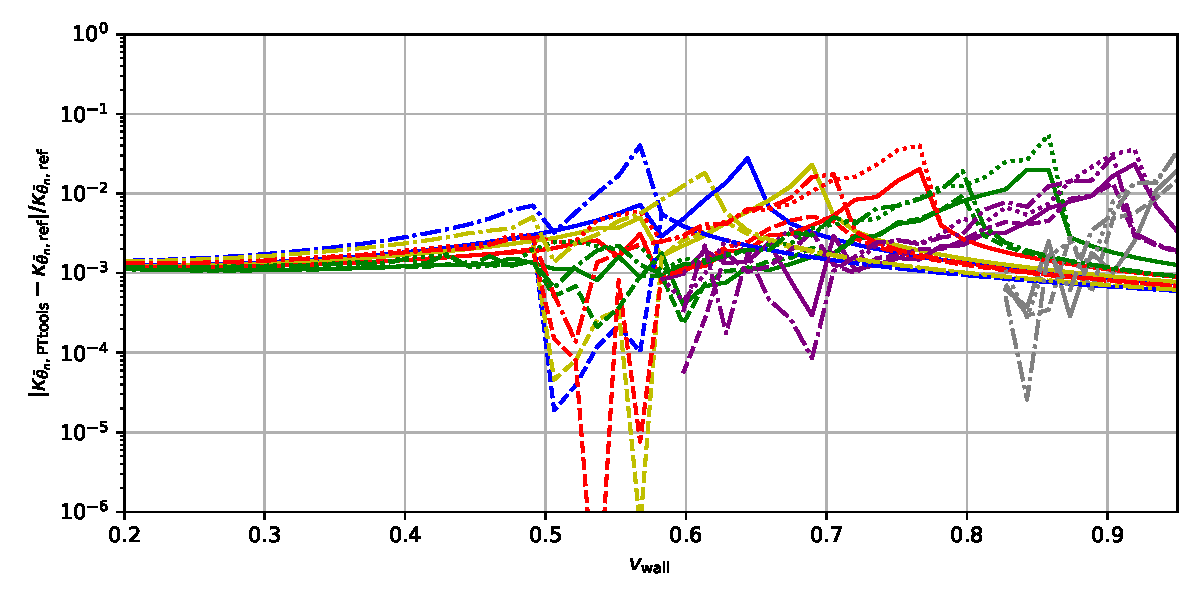
\includegraphics[width=\textwidth]{fig/giese_lisa_fig2_alpha_n_diff.pdf}
\caption{Relative difference of the $\kappa$ values by \cite[fig. 2]{giese_2021} and PTtools}
\label{fig:kappa_giese_diff}
\end{figure}

As we can see by the visually identical results in fig. \ref{fig:kappa_giese}
and the small scale of the relative differences in fig. \ref{fig:kappa_giese_diff},
the fluid profile simulations give nearly identical results.
This demonstrates that PTtools is a reliable fluid profile simulator for a variety of
sound speeds $c_s$, phase transition strengths $\alpha_n$ and wall speeds $v_\text{wall}$.
The differences are due to the differences in the number of the integration points chosen for the curve
and the different junction condition solver and ODE integration algorithms.

For $c_{s,s}=\frac{1}{4}$, $c_{s,b}=\frac{1}{3}$ and $\alpha_n = 0.01, 0.03$ the there is no curve,
as the $\alpha_n$ is below the theoretical minimum of $\alpha_n \approx 0.067$ for the model.
% The alpha_n_min was reported by pttools
This is recognised by the Giese et al. solver as well,
which is why it lacks the same curves.
% In \cite[fig. 2]{giese_2021} there are no such checks,
% which is why it has all these combinations.

The code by Giese et al. is specific to the constant sound speed model,
whereas the PTtools solver is desiged to be generic in such a way that
it can solve bubbles with arbitrary $c_s(T,\phi)$.
The PTtools code also enables easy extraction of various thermodynamic quantities,
and the gravitational wave spectra.
Therefore, now that we know that PTtools works reliably for the constant sound speed model,
the next step is to test it with more complex models.
